\documentclass[a4paper,12pt]{article}
\usepackage{amsmath}
\usepackage{amssymb}
\usepackage{graphicx}
%\documentclass{article}
\usepackage{setspace, enumitem,titlesec}
\usepackage{calc}
			% Activate to display a given date or no date
\usepackage{mathtools}
\usepackage{mathrsfs }
\DeclarePairedDelimiter\ceil{\lceil}{\rceil}
\DeclarePairedDelimiter\floor{\lfloor}{\rfloor}
\usepackage{algorithm}
\usepackage{algorithmic}
\usepackage{fancybox}

\usepackage{amsmath}
\usepackage{amssymb}
\usepackage{amsthm}
\usepackage{cite}
%\usepackage{algpseudocode}
\begin{document}
%\renewcommand{\thepseudonum}{\roman{pseudonum}}
\renewcommand\labelenumi{(\theenumi)}
%vector
\renewcommand{\vec}[1]{\mathbf{#1}}
\title {Review of Week 2 }
%\author{jim.morris.shen@gmail.com}
%\author{The Graduate Center, City University of New York}
\author{Xiaoke(Jimmy) Shen}
%\author{The Graduate Center, City University of New York}
\maketitle
%\textbf{Due Mar 1st 11:59 pm. 10 points for each exercise and 20 points for the extra credit exercise }\\
\section{Introduction}

This paper review report is provided based on the requirement of the computer science research course provided by the Graduate Center of the City University of New York during the 2017 Fall Semester. The main objective of this course is helping the PHD candidates to prepare their second exam and identify their thesis topic as early as possible\cite{ji2017}. \\

\section{Deep Learning Theory}

\subsection{Batch Normalization: Accelerating Deep Network Training by Reducing
               Internal Covariate Shift\cite{DBLP:journals/corr/IoffeS15}}
The main contribution of this paper as shown in Figure \ref{fig:bp} is it greatly reduced the convergence time for the training process and the BN(Batch Normalization) become one of the standard training step for the deep neural network after the publish of this paper.\\
\begin{figure}[H]
  \begin{center}
      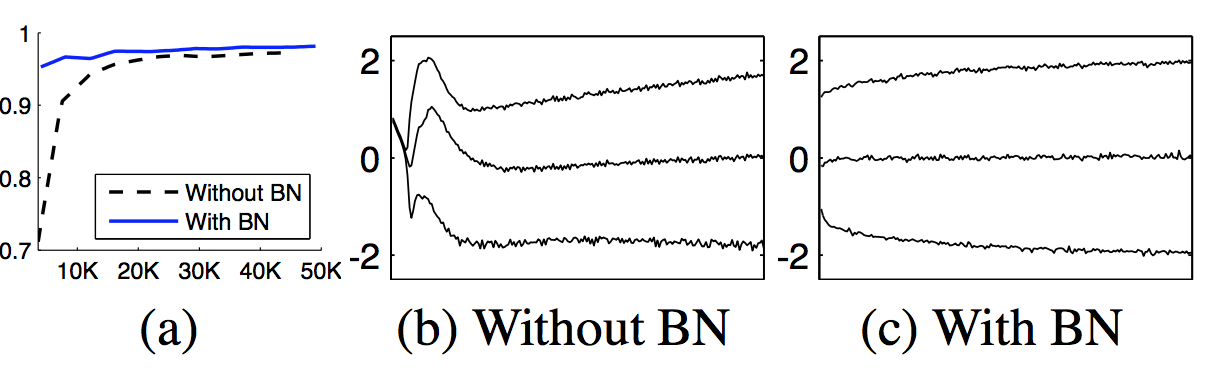
\includegraphics[scale=0.6]{bn.png}
\end{center}
\caption{(a) The test accuracy of the MNIST network trained with and without Batch Normalization, vs. the number of training steps. Batch Normalization helps the network train faster and achieve higher accuracy\cite{DBLP:journals/corr/IoffeS15}. (b, c) The evolution of input distributions to a typical sigmoid, over the course of training, shown as  15, 50, 85th percentiles. Batch Normalization makes the distribution more stable and reduces the internal covariate shift\cite{DBLP:journals/corr/IoffeS15}.}
 \label{fig:bp}
 \end{figure}

%\cite{Schmidhuber201585}

\section{Object Classification for 2D Images}
\subsection{Backpropagation applied to handwritten zip code recognition\cite{doi:10.1162/neco.1989.1.4.541}}
The first important application of using the BP(Back Propagation) to well resolve the real life problem from the literature. From this paper, one important structure of the neural network as show in Figure \ref{fig:bpzip} including the layers with filters were introduced. The similar structure is used in the modern neural network structures such as Alex Net\cite{NIPS2012_4824}, VGG 16  \cite{SimonyanZ14a} and resnet \cite{DBLP:journals/corr/HeZRS15}. The basic idea of the convolutional neural network was also introduced here.\\

\begin{figure}[H]
  \begin{center}
      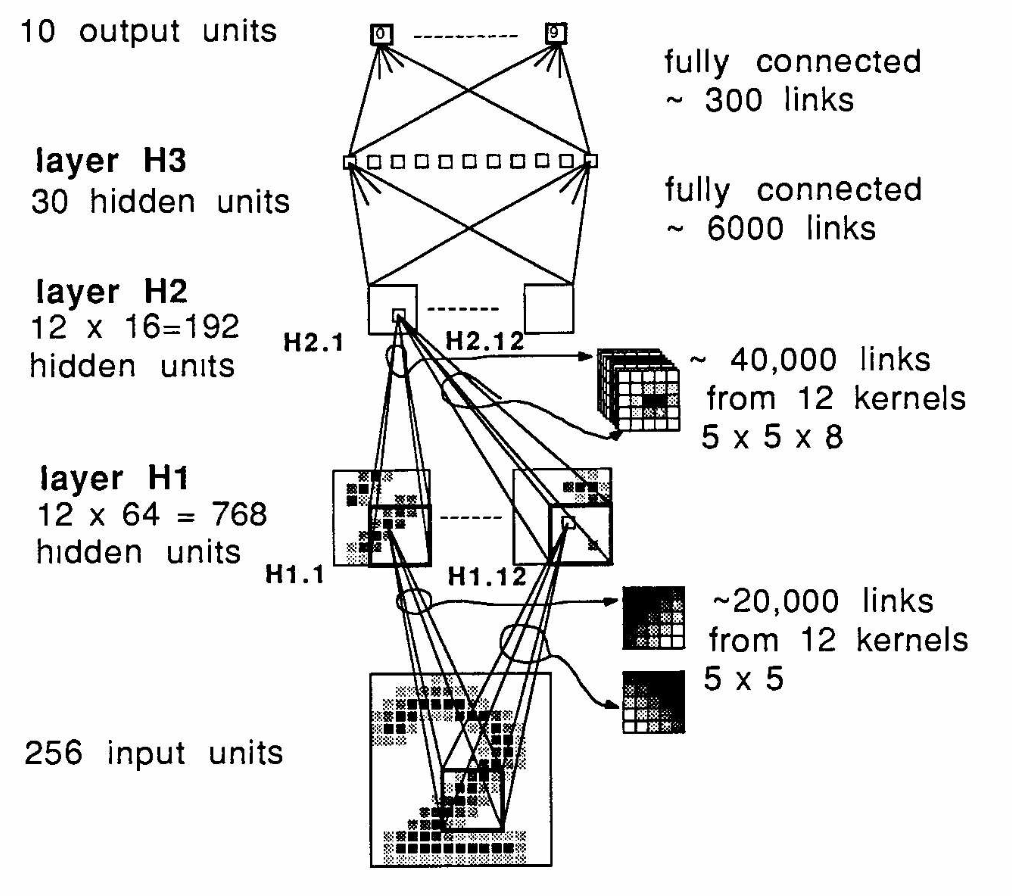
\includegraphics[scale=0.8]{bpzip.png}
\end{center}
\caption{The Neural Network used in \cite{doi:10.1162/neco.1989.1.4.541}.}
 \label{fig:bpzip}
 \end{figure}
 
\subsection{ImageNet: A Large-Scale Hierarchical Image Database\cite{imagenet_cvpr09}}
In the machine learning research area, two kinds of learning approaches can be done: supervised learning and unsupervised learning. For the supervised learning algorithms, the labeled data is required to train the algorithm. So the availability of the labeled data will become very important to the development of the supervised learning based algorithms. The ImageNet dataset \cite{imagenet_cvpr09} provides 1.2 million high-resolution labeled images of 1000 categories. This dataset becomes one of the most important datasets related to the object classification.\\


               
\bibliography{jimmy_shen}
\bibliographystyle{ieeetr}
  
 \end{document}